\documentclass{article}
\usepackage{geometry}
\geometry{a4paper}
\usepackage{amsmath}
\usepackage{empheq}
\usepackage{mhchem} % Package for chemical equation typesetting
\usepackage{siunitx} % Provides the \SI{}{} command for typesetting SI units
\usepackage{parskip}
\usepackage{graphicx} % Required for the inclusion of images
\usepackage{amssymb}
\usepackage{placeins}
\usepackage{cancel}
\usepackage{fullpage}
%\usepackage{subfig}
\usepackage{enumitem}
\usepackage{listings}
%\usepackage{mcode}
\usepackage{wrapfig}
%\renewcommand{\labelenumii}{\alph{enumi}.}
%Alph for uppcer case, \arabic for 1, 2, 3
%\roman for i, ii, iii \alph{enumi})
% Make numbering in the enumerate environment by letter rather than number (e.g. section 6)
\usepackage{booktabs, multicol, multirow}
%\usepackage[ ]{mcode} 

\setlength\parindent{0pt} % Removes all indentation from paragraphs

\renewcommand{\labelenumi}{\alph{enumi}.} % Make numbering in the enumerate environment by letter rather than number (e.g. section 6)

%\usepackage{times} % Uncomment to use the Times New Roman font



% Lots of macros. Thanks to D.F. Gleich for a bunch of these. 

\graphicspath{{./}{./figs/}}

  \def\clap#1{\hbox to 0pt{\hss#1\hss}}
  \def\mathclap{\mathpalette\mathclapinternal}
  \def\mathclapinternal#1#2{%
    \clap{$\mathsurround=0pt#1{#2}$}}

\usepackage{bm}
\providecommand{\mat}[1]{\bm{#1}}%
\renewcommand{\vec}[1]{\mathbf{#1}}
\newcommand{\vecalt}[1]{\bm{#1}}

% Commands
% bold upper case
\providecommand{\eye}{\mat{I}}
\providecommand{\mA}{\ensuremath{\mat{A}}}
\providecommand{\mB}{\ensuremath{\mat{B}}}
\providecommand{\mC}{\ensuremath{\mat{C}}}
\providecommand{\mD}{\ensuremath{\mat{D}}}
\providecommand{\mE}{\ensuremath{\mat{E}}}
\providecommand{\mF}{\ensuremath{\mat{F}}}
\providecommand{\mG}{\ensuremath{\mat{G}}}
\providecommand{\mH}{\ensuremath{\mat{H}}}
\providecommand{\mI}{\ensuremath{\mat{I}}}
\providecommand{\mJ}{\ensuremath{\mat{J}}}
\providecommand{\mK}{\ensuremath{\mat{K}}}
\providecommand{\mL}{\ensuremath{\mat{L}}}
\providecommand{\mM}{\ensuremath{\mat{M}}}
\providecommand{\mN}{\ensuremath{\mat{N}}}
\providecommand{\mO}{\ensuremath{\mat{O}}}
\providecommand{\mP}{\ensuremath{\mat{P}}}
\providecommand{\mQ}{\ensuremath{\mat{Q}}}
\providecommand{\mR}{\ensuremath{\mat{R}}}
\providecommand{\mS}{\ensuremath{\mat{S}}}
\providecommand{\mT}{\ensuremath{\mat{T}}}
\providecommand{\mU}{\ensuremath{\mat{U}}}
\providecommand{\mV}{\ensuremath{\mat{V}}}
\providecommand{\mW}{\ensuremath{\mat{W}}}
\providecommand{\mX}{\ensuremath{\mat{X}}}
\providecommand{\mY}{\ensuremath{\mat{Y}}}
\providecommand{\mZ}{\ensuremath{\mat{Z}}}
\providecommand{\mLambda}{\ensuremath{\mat{\Lambda}}}
\providecommand{\mSigma}{\ensuremath{\mat{\Sigma}}}
\providecommand{\mzero}{\ensuremath{\mat{0}}}
\providecommand{\mPsi}{\ensuremath{\mat{\Psi}}}
\providecommand{\mOmega}{\ensuremath{\mat{\Omega}}}

\providecommand{\ones}{\vec{e}}
\providecommand{\va}{\ensuremath{\vec{a}}}
\providecommand{\vb}{\ensuremath{\vec{b}}}
\providecommand{\vc}{\ensuremath{\vec{c}}}
\providecommand{\vd}{\ensuremath{\vec{d}}}
\providecommand{\ve}{\ensuremath{\vec{e}}}
\providecommand{\vf}{\ensuremath{\vec{f}}}
\providecommand{\vg}{\ensuremath{\vec{g}}}
\providecommand{\vh}{\ensuremath{\vec{h}}}
\providecommand{\vi}{\ensuremath{\vec{i}}}
\providecommand{\vj}{\ensuremath{\vec{j}}}
\providecommand{\vk}{\ensuremath{\vec{k}}}
\providecommand{\vl}{\ensuremath{\vec{l}}}
\providecommand{\vm}{\ensuremath{\vec{m}}}
\providecommand{\vn}{\ensuremath{\vec{n}}}
\providecommand{\vo}{\ensuremath{\vec{o}}}
\providecommand{\vp}{\ensuremath{\vec{p}}}
\providecommand{\vq}{\ensuremath{\vec{q}}}
\providecommand{\vr}{\ensuremath{\vec{r}}}
\providecommand{\vs}{\ensuremath{\vec{s}}}
\providecommand{\vt}{\ensuremath{\vec{t}}}
\providecommand{\vu}{\ensuremath{\vec{u}}}
\providecommand{\vv}{\ensuremath{\vec{v}}}
\providecommand{\vw}{\ensuremath{\vec{w}}}
\providecommand{\vx}{\ensuremath{\vec{x}}}
\providecommand{\vy}{\ensuremath{\vec{y}}}
\providecommand{\vz}{\ensuremath{\vec{z}}}
\providecommand{\vpi}{\ensuremath{\vecalt{\pi}}}
\providecommand{\vxi}{\ensuremath{\vecalt{\xi}}}
\providecommand{\vXi}{\ensuremath{\vecalt{\Xi}}}
\providecommand{\vmu}{\ensuremath{\vecalt{\mu}}}
\providecommand{\veps}{\ensuremath{\vecalt{\epsilon}}}
\providecommand{\vomega}{\ensuremath{\vecalt{\omega}}}
\providecommand{\vS}{\ensuremath{\vecalt{S}}}
% hats!
\newcommand{\hvc}{\hat{\vc}}
\newcommand{\hmA}{\hat{\mA}}
\newcommand{\hmC}{\hat{\mC}}
\newcommand{\hmG}{\hat{\mG}}
\newcommand{\hLambda}{\hat{\Lambda}}
\newcommand{\hTheta}{\hat{\Theta}}
\newcommand{\hmU}{\hat{\mU}}
\newcommand{\hmV}{\hat{\mV}}
\newcommand{\hmW}{\hat{\mW}}
\newcommand{\hlambda}{\hat{\lambda}}
\newcommand{\htheta}{\hat{\theta}}
\newcommand{\hvw}{\hat{\vw}}
\newcommand{\hvy}{\hat{\vy}}
\newcommand{\hvz}{\hat{\vz}}
\newcommand{\hpi}{\hat{\pi}}
\newcommand{\hY}{\hat{Y}}
\newcommand{\hZ}{\hat{Z}}
\newcommand{\hsY}{\hat{\mathcal{Y}}}

% tildes!
\newcommand{\mWt}{\tilde{\mW}}
\newcommand{\vwt}{\tilde{\vw}}
\newcommand{\vyt}{\tilde{\vy}}
\newcommand{\vzt}{\tilde{\vz}}

% script upper case
\newcommand{\sA}{\mathcal{A}}
\newcommand{\sB}{\mathcal{B}}
\newcommand{\sE}{\mathcal{E}}
\newcommand{\sI}{\mathcal{I}}
\newcommand{\sJ}{\mathcal{J}}
\newcommand{\sN}{\mathcal{N}}
\newcommand{\sL}{\mathcal{L}}
\newcommand{\sQ}{\mathcal{Q}}
\newcommand{\sR}{\mathcal{R}}
\newcommand{\sS}{\mathcal{S}}
\newcommand{\sX}{\mathcal{X}}
\newcommand{\sY}{\mathcal{Y}}
\newcommand{\sYt}{\tilde{\mathcal{Y}}}
\newcommand{\sZ}{\mathcal{Z}}

% script lower case
\newcommand{\sx}{\chi}

% bold greek
\newcommand{\balpha}{\bm{\alpha}}
\newcommand{\feta}{\bm{\eta}} % \feta is for ``fat eta''
\newcommand{\bpi}{\bm{\pi}}
\newcommand{\btheta}{\bm{\theta}}
\newcommand{\bOmega}{\bm{\Omega}}
\newcommand{\bomega}{\bm{\omega}}
% some useful commands
\newcommand{\ip}[2]{\left\langle #1,\,#2\right\rangle}
\newcommand{\Exp}[1]{\mathbb{E}\left[#1\right]}
\newcommand{\parens}[1]{\left(#1\right)}
\newcommand{\braces}[1]{\left\lbrace #1 \right\rbrace}
\newcommand{\brackets}[1]{\left[ #1 \right]}
\newcommand{\CExp}[2]{\mathbb{E}\left[#1\,|\,#2\right]}
\newcommand{\Cov}[2]{\operatorname{Cov}\left[#1,\,#2\right]}
\newcommand{\Corr}[2]{\operatorname{Corr}\left[#1,\,#2\right]}
\newcommand{\Var}[1]{\operatorname{Var}\left[#1\right]}
\newcommand{\Prob}[1]{\mathbb{P}\left[#1\right]}
\newcommand{\bmat}[1]{\begin{bmatrix}#1\end{bmatrix}}
\newcommand{\ddx}[2]{\frac{\partial #1}{\partial x_{#2}}}
\newcommand{\argmax}[1]{\underset{#1}{\mathrm{argmax}}}
\newcommand{\argmin}[1]{\underset{#1}{\mathrm{argmin}}}
\newcommand{\mini}[1]{\underset{#1}{\mathrm{minimum}}}
\newcommand{\maxi}[1]{\underset{#1}{\mathrm{maximum}}}
\newcommand{\st}{\text{subject to }}
\newcommand{\trace}[1]{\operatorname{trace}\left(#1\right)}
%\newcommand{\grad}[2]{\nabla_{#2} #1}
\newcommand{\gf}{\nabla_\vx f}
\newcommand{\intrho}[1]{\int #1 \,\rho\,d\vx}
\newcommand{\lmax}{\lambda_{\text{max}}}
\newcommand{\ran}[1]{\operatorname{ran}(#1)}
\newcommand{\dist}[2]{\operatorname{dist}(\ran{#1},\,\ran{#2})}
\newcommand{\verteq}{\rotatebox{90}{$\;\equiv\;$}}
\newcommand{\vertap}{\rotatebox{90}{$\;\approx\;$}}
\newcommand{\diag}[1]{\operatorname{diag}(#1)}
\newcommand{\sspone}[2]{\operatorname{SSP}(#1,#2)}
\newcommand{\ssptwo}[3]{\operatorname{SSP}(#1,#2,#3)}
\newcommand{\myspan}[1]{\operatorname{ran}(#1)}
\newcommand{\ymax}{y_{\text{max}}}
\newcommand{\Pmax}{P_{\text{max}}}
\newcommand{\vol}[1]{\operatorname{Vol}(#1)}
\newcommand{\pone}[2]{\frac{\partial #1}{\partial #2}}
\newcommand{\ptwo}[2]{\frac{\partial^2 #1}{\partial #2^2}}
\newcommand{\pthree}[2]{\frac{\partial^3 #1}{\partial #2^3}}
\newcommand{\pfour}[2]{\frac{\partial^4 #1}{\partial #2^4}}
\newcommand{\done}[2]{\frac{d #1}{d #2}}
\newcommand{\dtwo}[2]{\frac{d^2 #1}{d #2^2}}
\newcommand{\dthree}[2]{\frac{d^3 #1}{d #2^3}}
\newcommand{\dfour}[2]{\frac{d^4 #1}{d #2^4}}
% theorem environments
\newtheorem{assumption}{Assumption}

% for bayesian inversion
\newcommand{\prior}{\rho_{\text{pr}}}
\newcommand{\priory}{\rho_{\text{pr},Y}}
\newcommand{\priorz}{\rho_{\text{pr},Z}}
\newcommand{\lik}{\rho_{\text{lik}}}
\newcommand{\post}{\rho_{\text{post}}}
\newcommand{\postt}{\tilde{\rho}_{\text{post}}}
\newcommand{\posty}{\rho_{\text{post},Y}}
\newcommand{\cprior}{c_{\text{pr}}}
\newcommand{\cpost}{c_{\text{post}}}
\newcommand{\cpostt}{\tilde{c}_{\text{post}}}
\newcommand{\dcov}{\Gamma_{\vd}}


% File path abrev
%\newcommand{\ip}[2]{\left\langle #1,\,#2\right\rangle}

\newcommand{\figpath}[1]{code/figs/crops/#1}

%\braces , \parens \brackets \mC (matrix C) \vv (vector v) \h hats for somethings ie \hvy or \hmA \sA (subscript upper case)
\usepackage{caption}
\usepackage{subcaption}

%----------------------------------------------------------------------------------------
%	DOCUMENT INFORMATION
%----------------------------------------------------------------------------------------
%$\frac{-1}{\sqrt{a}}$
%\title{Newberry/Felix  \hfill \today}
%\date{}
\begin{document}
%\maketitle 
%\LARGE
\textsc{\Large Structure Solver Variational form \hfill \today}\\[0.5cm] % Name of your university/college

The derivation of variational form for dynamic nonlinear elasticity is derived. The method described is detailed in chapters 28 and 29 of the FEniCS book. 

The structure body in question is idealized to be described by $\Omega$ points in the body.  The problem is considered in a Lagrangian description with reference positions $X \in \Omega$. We introduce $\varphi$, a continuously differentiable one to one map, to describe the displacement field  

\begin{equation}
u(X,t) = \varphi (X,t) - X
\end{equation}

where the displacement $u$ for a given point in time is measured relative to the known reference position $X$. 
$\partial \Omega$ is the boundary of $\Omega$. 

The solution of our displacement field depends on three categories of boundary conditions:

\begin{itemize}
\item Body forces that act on the entire volume of the body: $B(X,t)$
\item Traction forces, force per unit area on the Neumann boundary: $\partial \Omega_N$
\item Displacement, prescribed displacement boundary conditions on the Dirichlet boundary: $\partial \Omega_D$
\end{itemize}

Figure \ref{fig:structure} depicts a generic structure body and associated boundary conditions. 

\FloatBarrier
\begin{figure}[h]
\centering
	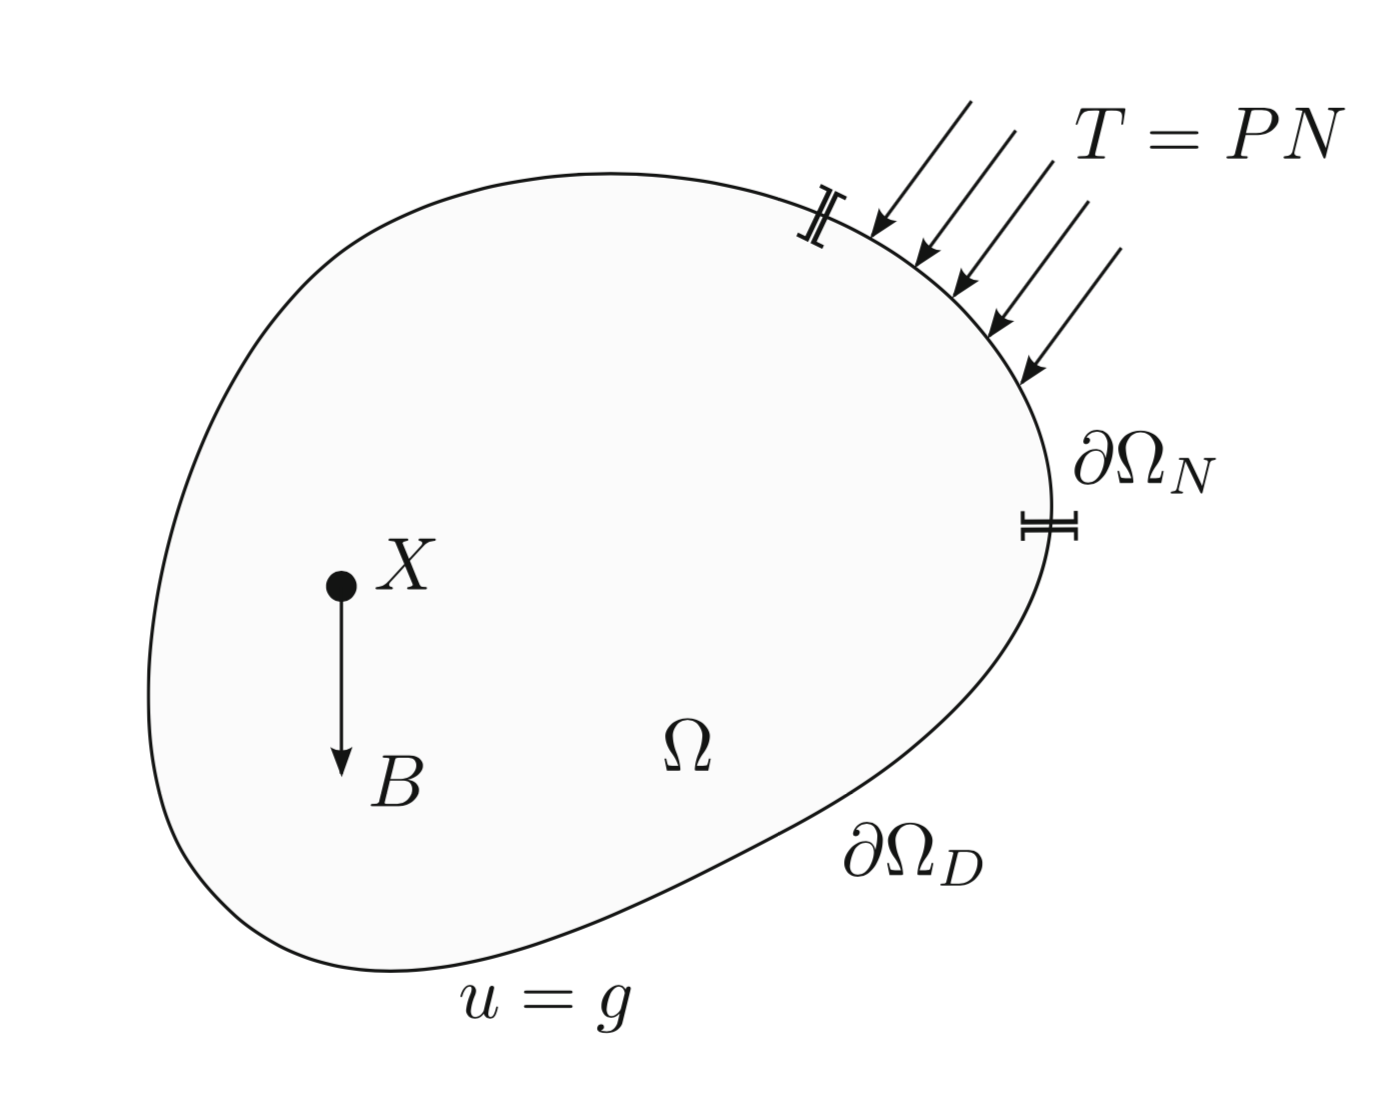
\includegraphics[width=0.4\textwidth]{structure}
	\caption{Structure body subject to body force, traction on the Neumann boundary and prescribed displacement on the Dirichlet boundary. \cite{logg2012automated} }
	\label{fig:structure}
\end{figure}
\FloatBarrier

Demonstrated in Figure \ref{fig:structure}, we assume that the Neumann and Dirichlet boundaries do not coincide. 

Beginning with the Lagrangian form of the balance of linear momentum: 

\begin{equation}
\rho \ptwo{u}{t} = Div (P) + B \: \text{in} \: \Omega
\label{eqn:lagrangian}
\end{equation}

where $\rho$ is the density of the structure, $P$ the first Piola-Kirchoff stress tensor and B the body force per unit volume. 

We define initial conditions $u(X,0) = u_0(X)$ and $\pone{u}{t}(X,0) = v_0(X)$ and boundary conditions $u(X,t) = g(X,t)$ on $\partial \Omega_D$ and $P(X,t) N(X) = T(X,t)$ on $\partial \Omega_N$. $N(X)$ is the outward normal to the boundary at point $X$. 

We take the dot product of \ref{eqn:lagrangian} with a test function $v \in \hat{V}$ and integrate over the reference domain and time to arrive at 

\begin{equation}
\int_{0}^{T} \int_{\Omega} \rho \ptwo{u}{t} \cdot v \; dx  \; dt  = \int_{0}^{T} \int_{\Omega} Div(P) \cdot v \; dx \; dt + \int_{0}^{T} \int_{\Omega} B \cdot v \; dx \; dt 
\end{equation}

Next, apply the divergence theorem to arrive at the weak form the balance of linear momentum. We introduce the traction vector $T = PN$ on the Neumann boundary $\partial \Omega_N$ and use $v = 0$ on $\partial \Omega_D$, by definition of the Dirichlet boundary. This yields a weak form. Find $u \in V$ such that $ \forall \;  v \in \hat{V}$:
   
\begin{equation}
\int_{0}^{T} \int_{\Omega} \rho \ptwo{u}{t} \cdot v \; dx  \; dt + \int_{0}^{T} \int_{\Omega} P: Grad(v) \; dx \; dt = \int_{0}^{T} \int_{\Omega} B \cdot v \; dx \; dt + \int_{0}^{T} \int_{\partial \Omega_N} T \cdot v \; ds \; dt 
\label{eqn:weak_1}
\end{equation}

The dynamic approach taken here is $CG_1$ meaning the finite element space $V$ is continuous and piecewise linear in time. We rewrite \ref{eqn:weak_1}, which is 2nd order in time, as a system of first order equations with the variable $w = \pone{u}{t}$. This yields a new weak form. Find $(u, w) \in V$, such that $\forall \; (v,r) \in \hat{V}$:

\begin{align}
\int_{0}^{T} \int_{\Omega} \rho \pone{w}{t} \cdot v \; dx  \; dt + \int_{0}^{T} \int_{\Omega} P: Grad(v) \; dx \; dt &= \int_{0}^{T} \int_{\Omega} B \cdot v \; dx \; dt + \int_{0}^{T} \int_{\partial \Omega_N} T \cdot v \; ds \; dt \hspace{1cm} \text{and} \\
\int_{0}^{T} \int_{\Omega} \pone{u}{t} \cdot r \; dx \; dt &= \int_{0}^{T} \int_{\Omega} w \cdot r \; dx \; dt. 
\end{align}

with the initial conditions established earlier as $u(X,0) = u_0(X)$ and $w(X,0) \pone{u}{t} (X,0) = v_0(X)$ in $\Omega$ and boundary conditions $u(X,t) = g(X,t)$ on $\partial \Omega_D$. While the displacement finite element approximation space is $CG_1$, the velocity space $\hat{V}$ is $DG_0$, discontinuous and piecewise constant in time. This produces

\begin{align}
\int_{\Omega} \rho \frac{(w_{n+1} - w_n)}{\Delta t} \cdot v \; dx  + \int_{\Omega} P (u_{mid}): Grad(v) \; dx  &=  \int_{\Omega} B \cdot v \; dx + \int_{\partial \Omega_N} T \cdot v \; ds  \hspace{1cm} \text{and} \\
\int_{\Omega} \frac{(u_{n+1} - u_n)}{\Delta t} \cdot r \; dx  &= \int_{\Omega} w_{mid} \cdot r \; dx 
\end{align}

where $(\cdot)_n$ and $(\cdot)_{n+1}$ denote a quantity at the previous and current time step, and $(\cdot)_{mid} = \frac{((\cdot)_n +(\cdot)_{n+1})}{2}$. 

In FEniCS this equation is solved in a mixed function space with Netwon's method. Each term is multiplied by $\Delta t$ and $Piola-Kirchoff$ stress is calculated from $(u)_{mid}$.

 To arrive at this variational form the first Piola-Kirchhoff stress tensor must be found. The necessary kinematic terms to determine the first Piola-Kirchhoff stress are presented in Table \ref{tab:kinematics}

\FloatBarrier
  \begin{table}[htbp]
  \setlength\extrarowheight{5pt}
  \centering
  \caption{Kinematic terms}
    \begin{tabular}{cc}
    Deformation Gradient & $F = I + Grad(u)$\\
    Right Cauchy-Green tensor & $C = F^T F$ \\
    Green-Lagrange strain tensor & $E = \frac{1}{2}(C - I)$ \\
    \end{tabular}%
  \label{tab:kinematics}%
\end{table}%
\FloatBarrier

For the benchmark FSI problem, the material model employed is St Venant Kirchhoff with a stored strain energy of 

\begin{equation}
\Psi = \frac{\lambda}{2} tr(E^2) + \mu tr(E^2) 
\end{equation}

where $\mu$ and $\lambda$ are the structure first and second lame constants respectively. Given $\Psi$ is dependent on the Green-Lagrange tensor the second Piola-Kirchhoff stress can be calculated as.

\begin{equation}
S = \pone	{\Psi (E)}{E} 
\end{equation}

From this the first Piola-Kirchoff stress is found as

\begin{equation}
P = FS
\end{equation}

Excluding the traction, this implementation has been validated against a benchmark in FEniCS. I'm therefore confident of the derivation and implementation of the first Piola-Kirchohhoff stress in the dynamic code. 

Addressing the traction. 

The Cauchy stress tensor of the fluid problem is calculated as

\begin{equation}
\sigma = -p I + \mu_f (grad(u_f) + grad(u_f)^T )
\end{equation}
where $p$ is the fluid pressure, $\mu_f$ the dynamic viscosity and $u_f$ the fluid velocity. This stress is projected onto a tensor function space in the structure domain. 

The traction is then calculated.

The fluid traction is transferred to the structure via the Piola map
$$ (j \sigma_F \cdot f^{-T}) \cdot n_f = -\sigma_s \cdot n_s $$
where $j = det (f)$ is the determinant of the Jacobi matrix $f = grad(\varphi)$ and $n_f$ and $n_s$ are the respective fluid and structure mesh facet normals. $\varphi$ is defined earlier relating to the structure displacement as $u(X,t) = \varphi (X,t) - X$. My current FEniCS implementation reads $f = grad(\varphi) = grad(u)+ I$. 
I'm not confident on the reasoning implicit here that $grad(X) = I$. 

My understanding is that the implementation I have in FEniCS follows the book closely. At the moment when I run 

\bibliography{validation}{}
\bibliographystyle{plain}

\end{document}
